%!TEX root=rapport.tex
\section{Implémentation}

\subsection{Idée générale}

	L'idée générale de l'alignement de séquences est de permettre à partir d'un ensemble de séquences de créer à l'aide de chevauchements approximatifs un \emph{contig}. Pour se faire, notre démarche se découpe en plusieurs parties:

	\begin{description}
		\item[Récupération et stockage des données] Afin de pouvoir former le contig souhaité, il est nécessaire de récupérer les séquences et de les stocker de manière efficace. Cette étape est expliquée dans la section~\ref{subsection:recStock}.

		\item[Alignement semi-global] Ensuite, pour chaque paire de séquence,
			nous effectuons un \emph{alignement semi-global} en nous inspirant
			de l'algorithme vu en cours. Cette méthode nous donne ainsi
			l'alignement approximatif des deux séquences, ce qui permet de
			prendre en compte le fait qu'il ait pu y avoir des erreurs lors du
			séquençage. Si la paire est noté $(s, t)$, cette étape nous permet également de connaitre la plus
			grande chaine qui est suffixe de $s$ et préfixe de $t$. Cette étape
			est expliquée dans la section~\ref{subsection:semiGlobal}.

		\item[Algorithme greedy] Une fois les alignements approximatifs
			calculés, il est encore nécessaire de trouver dans quel ordre
			ceux-ci doivent être assemblés afin de former le meilleur contig.
			Pour se faire, nous utilisons un \emph{algorithme greedy} qui, à
			partir d'un graphe permet de trouver un chemin hamiltonien afin de
			reconstituer le contig. Cette étape est expliquée dans la
			section~\ref{subsection:greedy}.

		\item[Alignement]
			L'algorithme greedy nous donnant, dans l'ordre, les séquences à
			aligner, il est nécessaire de reconstruire cet alignement en
			ajoutant des gaps pour que chaque séquence ait la même longueur et
			qu'on puisse calculer le consensus. Cette étape est expliquée dans
			la section ~\ref{subsection:alignment}.

		\item[Consensus]
			Maintenant que l'alignement a été réalisé, il nous faut calculer le
			consensus en fonction de ce dernier. Cette étape est expliquée dans
			la section ~\ref{subsection:consensus}.
	\end{description}

\subsection{Récupération et stockage des données}
\label{subsection:recStock}

Cette étape est effectuée au travers des classes \verb|FastaReader| et \verb|Alignement|. De plus, la classe \verb|FastaWriter| est utilisée afin de récupérer le résultat du procédé visant à trouver le meilleur contig.\\

La classe \verb|Alignment| permet de stocker sous forme d'un table de Bytes un fragment d'ADN. Nous prenons la convention suivante quant à la représentation des nucléotides et d'un gap:
	\begin{center}
		\begin{tabular}{|l|c|}
			\hline
			Nucléotide/Gap & Représentation \\
			\hline
			\hline
			C & 0 \\
			\hline
			G & 1\\
			\hline
			T &  2 \\
			\hline
			A &  3 \\
			\hline
			Gap & 4 \\
			\hline

		\end{tabular}
	\end{center}

	Le fait de stocker les nucléotides sous forme de Bytes permet de réduire l'espace mémoire nécessaire.

	  Elle contient également des méthodes intéressantes telles que \textsc{complement} qui permet de complémenter et inverser une séquence d'ADN ainsi que d'autres méthodes comme \textsc{backTrack} et \textsc{semiGlobalAlignment} qui sont utiles pour l'étape décrite dans la section~\ref{subsection:semiGlobal} ou encore \textsc{arcGenerator} qui est expliquée dans la section~\ref{subsection:greedy}.\\

La classe \verb|FastaReader| permet à partir d'un \emph{fichier Fasta} de générer un liste d'objets \verb|Sequence| représentant les fragments d'ADN. \\

L'opération inverse est possible grâce à la classe \verb|FastaWriter|.





\subsection{Alignement semi-global}
\label{subsection:semiGlobal}

Une des premières étapes de la démarche est d'effectuer l'alignement semi-global
entre deux fragments. Cette étape permet de tester la similarité entre les deux
fragments que l'on veut aligner. L'alignement semi-global est implémenté dans la
classe \verb|Sequence| via la fonction \textsc{semiGlobalAlignement}. Cette
méthode prend deux fragments $f$ et $g$, des coûts de match, missmatch et gap
et calcule l'alignement tel que $f$ précède $g$ (alignement de type ($f,g$))et celui tel que $g$ précède $f$ (alignement de type ($g,f$)) et
renvoie le résultat sous forme d'une liste de \verb|SequenceAlignement|. Ce comportement est un peu différent de celui du cours, 
car dans ce dernier on se contentait de garder le meilleur des deux alignements. Ici nous sommes intéressés à la fois  au meilleur alignement suffixe-prefixe de $f$ avec $g$ mais également le cas inverse ($g$ avec $f$). Ces deux situations sont illustrés à la figure~\ref{fig:alignementType}.
On remarque que lorsque l'on calcule la matrice de similarité, si le fragment $f$ est placé sur l'axe vertical et si le fragment $g$ est placé sur l'axe horizontal, on trouve le score d'alignement de type $(f,g)$ en prenant le maximum sur la dernière ligne de la matrice. En effet, cela signifie que l'on a parcouru tous les éléments de la séquence $f$ avant de finir le parcours des éléments de la séquence $g$. De la même manière on trouve les alignements de type $(g,f)$ en prenant le maximum de la dernière colonne de la matrice.\\

\begin{figure}
	\begin{minipage}[r]{.46\linewidth}
		\begin{center}
		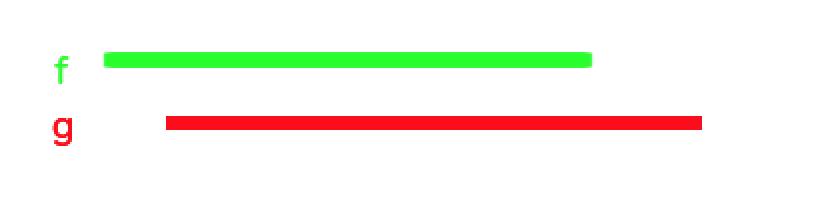
\includegraphics[scale= 0.50]{(f,g).png}
		Alignement de type (f,g)
	\end{center}
	   \end{minipage} \hfill
	   \begin{minipage}[c]{.46\linewidth}
		\begin{center}
			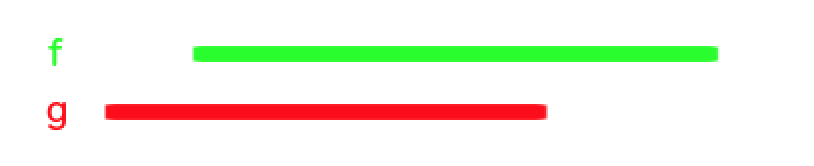
\includegraphics[scale= 0.50]{(g,f).png}
			Alignement de type (g,f)
		\end{center}
			  \end{minipage}
		\caption{Alignements résultants de l'alignement de f et de g}
		\label{fig:alignementType}
\end{figure}


Un objet de la classe \verb|SequenceAlignement| est défini de la manière
suivante: le segment $f$ aligné avec le segment $g$ en supposant que le
segment $f$ est le segment le plus à \og gauche \fg. De plus, la longueur du
préfixe-suffixe commun est stocké dans l'attribut \emph{longestCommonSubstringLength} ainsi que le score d'alignement dans l'attribut \emph{score}.\\

De plus, dans la classe \verb|Sequence| nous retrouvons la méthode \emph{arcGenerator} qui à partir de deux fragments $f$ et $g$ calcule tous les alignements possibles. C'est-à-dire, si on considère que $\overline{f}$ est le fragment complémentaire inversé de $g$, alors on calcule:\\
\begin{itemize}
	\item[$\bullet$] L'alignement $(f,g)$ ainsi que $(g,f)$;
	\item[$\bullet$] L'alignement de $(\overline{f},g)$ ainsi que $(g, \overline{f})$;
	\item[$\bullet$] L'alignement de $(f, \overline{g})$ ainsi que $(\overline{g},f)$;
	\item[$\bullet$] L'alignement de $(\overline{f}, \overline{g})$ ainsi que $(\overline{g}, \overline{f})$.
\end{itemize}
$ $\\
Au vu des explications ci-dessus, il est important de remarquer que pour trouver les 8 alignements il n'est nécessaire de calculer uniquement 4 matrices de similarités (une pour chaque paire de l'énumération ci-dessus).\\

A partir de ces alignements nous construisons les objets \verb|Arc|. Un objet arc possède en attribut:\\

\begin{itemize}
	\item[$\bullet$] Les fragments $f$ et $g$ initiaux qui sont utilisés lors de l'alignement. Ceux sont stockés dans des attributs \emph{start} et \emph{end} pour savoir respectivement s'il s'agit de l'origine ou de l'extrémité de l'arc.
	\item[$\bullet$] Des booléens relatifs à $f$ et $g$ (un pour chacun) qui permettent de savoir si on considère le complémentaire inversé lors de l'alignement.
	\item[$\bullet$] Le score correspondant à l'alignement.
	\item[$\bullet$] Un booléen \emph{inside} qui permet de déterminer si lors de l'alignement un des deux fragments est inclus à l'autre.
	
\end{itemize}

Nous pouvons remarquer que nous ne stockons pas, l'alignement résultant de l'alignement semi-global. En effet, comme à la fin du procédé le nombre d'alignements réels qui nous intéressent sont au nombre de $n-1$ (si $n$ est le nombre de fragments total), il n'est pas nécessaire de stocker en mémoire tous les alignements possibles. Dans le but de gagner en mémoire, nous préférons dès lors recalculer l'alignement correspondant aux arcs choisis par l'algorithme greedy. Ceci est réalisé par le biais de la méthode \

Ces arcs nous permettent d'effectuer l'algorithme greedy pour trouver un chemin hamiltonien parcourant tous les fragments considérés.


\subsection{Algorithme greedy}
\label{subsection:greedy}

Avant de nous intéresser à l'algorithme greedy en tant que tel, nous allons expliquer une structure de données \emph{Union-Find} que nous utilisons pour l'implémentation de cet algorithme.

\subsubsection{Union-Find}

Une structure de donnée \og Union-Find \fg~est une structure permettant de représenter une relation d'équivalence . On peut effectuer trois opérations sur cette structure:
\begin{itemize}
\item[$\bullet$] L'opération \textsc{Find} permet de déterminer dans quelle classe d'équivalence se situe un élément.
\item[$\bullet$] L'opération \textsc{Union} permet de faire l'union entre deux classes d'équivalence.
\item[$\bullet$] L'opération \textsc{MakeSet} construit une classe d'équivalence qui ne contient qu'un seul élément
\end{itemize}

Dans l'implémentation que nous avons utilisée, chaque classe d'équivalence est représentée par un arbre pour lequel chaque noeud possède une référence vers son père. Dans un tel choix d'implémentation, la racine de chaque classe correspond au représentant de la classe d'équivalence.

L'idée est que l'opération \textsc{Find} permet de retourner à la racine de l'arbre et donc de déterminer quel est le représentant de la classe d'équivalence. Pour l'opération \textsc{Union}, on rattache la racine d'une des deux classes à celle de l'autre classe. Toutefois, une telle démarche pourrait amener à des arbres fortement déséquilibrés . Afin d'éviter cela, une heuristique sur la hauteur de l'arbre est utilisée. On retient le \emph{rang} de l'arbre et à chaque fois que l'on veut faire l'union de deux arbres on considère leur rang. On attache l'arbre de rang inférieur à la racine de l'arbre de rang supérieur. Les arbres qui ne contiennent qu'un seul élément sont de rang 0 et dès que l'on effectue l'union de deux arbres de même rang, le résultat de cette union a un rang d'une unité plus grand.

\todo{ un mot sur la complexité?}

\subsubsection{Recherche du chemin hamiltonien}

Afin de trouver la meilleure séquence finale, nous devons trouver un chemin hamiltonien de poids maximal dans le graphe composé des arcs dont la construction est décrite dans la section~\ref{subsection:semiGlobal}. Le déroulement général de l'algorithme greedy est le suivant: à chaque étape d'exécution de l'algorithme, l'algorithme sélectionne et retire l'arc de poids le plus élevés d'un ensemble d'arcs. Plusieurs critères doivent alors être vérifiés pour savoir si l'arc doit être retenu. Si l'arc est l'arc $(f,g)$ où $f$ est l'origine de l'arc et $g$ son extrémité, il faut vérifier qu'on ne soit pas déjà rentré dans le \og noeud \fg~$g$ ni qu'on ne soit déjà sorti du \og noeud \fg~$f$, de plus, il faut s'assurer que $f$ et $g$ ne fasse pas déjà partie de la même classe d'équivalence. Vu que dans notre cas, nous travaillons également avec le complémentaire inversé, il faut s'assurer que lorsqu'un fragment $f$ est choisi pour la formation du chemin hamiltonien, il n'est pas possible de considérer son complémentaire inversé $\overline{f}$.

La mise en oeuvre de l'algorithme greedy se trouve dans la classe \verb|Greedy|. Nous détaillons ci-dessous le rôle des différentes méthodes qui s'y trouvent.

\begin{description}
	\item[\textsc{generateAllPairs}] Cette méthode permet à partir d'une liste d'objets \verb|Sequence| de générer toutes les paires de séquences qui devront être considérés.
	\item[\textsc{isAcceptable}] Pour un arc donné, cette méthode permet de déterminer si cet arc suit les conditions d'acceptabilités expliquées ci-dessus. 
	\item[\textsc{filterArcs}] C'est au sein de cette méthode que l'algorithme greedy comme décrit dans le cours est effectué. A partir d'une liste d'arcs, on calcule les sequences ayant générés ces arcs afin de pouvoir générer la structure d'\verb|Union-find|. Deux ensembles \emph{entered} et \emph{exited} permettent de tenir à jours les \og noeuds \fg~dans lesquels on est rentré ou sorti. Une autre structure \emph{comp} permet de savoir déterminer si on a déjà utilisé un fragment et si oui, s'il est utilisé sous sa forme complémentée inversée ou pas. L'algorithme choisit à chaque fois l'arc de poids le plus élevé et teste s'il est acceptable. Si oui, on ajoute cet arc pour la construction du chemin hamiltonien et on met à jour toutes les structures décrites précédemment et on choisit un nouvel arc. Si non, on choisit directement un nouvel arc.
	\item[\textsc{hamiltonianPath}] A partir de l'ensemble des arcs acceptés par la méthode \emph{filterArcs} reconstruit le chemin hamiltonien sous forme d'une liste d'arcs.
	\item[\textsc{greedy}] Cette méthode rassemble toutes les méthodes précédentes. On commence par générer toutes les paires de séquences possibles. A partir de cela, nous construisons les arcs. C'est à cet endroit que le travail est le plus couteux (car il demande de calculer les matrices de similarité). C'est pourquoi nous parallélisons cette étape. Nous avons ensuite la possibilité de retenir certains arcs selon certains critères. Nous avons tenter de rejeter les arcs qui correspondaient un alignement de type \og inside \fg. Les tests effectués après cette modification semblant donner des résultats moins bons, cette alternative n'a pas été retenue. Nous n'avons dès lors à ce jour, pas encore trouvé de moyen efficace de traiter les alignements de type \og inside \fg. Nous construisons ensuite le chemin hamiltonien d'arcs. Toutefois, les alignements n'étant pas stocké dans les arcs, nous devons recalculer les alignements entre les deux séquences. Cela se fait via le biais de la fonction \emph{getAlignement} de la classe \verb|Arc|. 
	Ensuite, on renvoie le chemin hamiltonien de \verb|SequenceAlignment| qui est ainsi prêt à être utilisé pour retrouver la séquence finale.	
	\end{description}
\subsection{Alignement}
\label{subsection:alignment}
Les deux dernières étapes que sont l'alignement et le consensus sont 
implémentées dans la classe \verb|ConsensusAbstract| à travers les méthodes 
\verb|computeAlignment| qui calcule l'alignement des séquences et le sauvegarde 
dans l'attribut \verb|alignment| ainsi qu'à travers la méthode \verb|build| 
qui calcule le consensus.

Pour calculer l'alignement, nous utilisons les segments alignés ans l'ordre 
donné par l'algorithme greedy décrit à l'étape \ref{subsection:greedy}.
L'algorithme greedy nous ressort une liste de paires de séquences $P_{i}$ tel
que le deuxième segment de la paire $P_{i}$ provient du même segment initial que
le premier de la paire $P_{i + 1}$, la différence se situant dans les gaps
ajoutés lors de l'alignement semi-global entre les nucléotides pour offrir le
meilleur score pour chaque paire.

Pour pouvoir construire le contig final, il nous faut réaligner convenablement
chaque paire de segments et pour cela, nous allons propager les gaps qui ont été
ajoutés lors des calculs de l'alignement semi-global. Nous effectuons cette
propagation en deux temps:

\begin{enumerate}
	\item vers le bas, c'est-à-dire, pour une paire $P_{i}$ on regarde si, entre
		deux nucléotides de la deuxième composante de $P_{i}$, le
		nombre de gaps est plus grand qu'entre les deux mêmes nucléotides de la première
		séquence de la paire suivante $P_{i + 1}$ et si c'est le cas, on propage la
		différence entre ces nombres vers les séquences du dessous.
	\item vers le haut par le même procédé que pour la propagation vers le bas
		sauf que nous propageons les gaps qui sont plus présents dans la
		première composante de la paire $P_{i + 1}$ que dans la deuxième
		composante de paire $P_{i}$ et qu'on propage alors la différence de gaps
		vers les séquences du dessus.
\end{enumerate}

Grace à ce procédé, nous sommes sûrs que les séquences résultantes des
alignements semi-globaux sont bien les mêmes et que l'ordre renvoyé par le greedy
est toujours le même (car l'ordre des scores reste le même).

\subsubsection{Représentation d'une séquence pour l'alignement}

Au vu de cette méthode de propagation de gaps, le procédé d'alignement n'est
donc qu'un ajout de gaps entre nucléotides: il est alors intéressant de
représenter les séquences alignées comme des séquences sans gaps où, après
chaque nucléotide de la séquence, nous retenons, dans un tableau d'entier, le
nombre de gaps suivant celui-ci.\footnote{Une même représentation peut être
	utilisée pour représenter pour les nucléotides successifs identiques: nous
	compressons ainsi la séquence. Nous n'avons souhaité compresser que les gaps
	car nous n'allons travailler qu'avec ceux-ci, et cela aurait complexifié
l'implémentation des méthodes.}

Par exemple, la séquence \verb|A--T-G-C| sera représenté par une séquence
\verb|ATGC| et par un tableau nommé \verb|nb_gaps| de taille 4
contenant les entiers {2, 1, 1, 0} car il y a deux gaps après le premier
nucléotide, un gap après le second, un après le troisième, et 0 à la fin. Les
complexités en temps et en mémoire sont ainsi diminuées.
Au niveau de la mémoire, une séquence alignée se voit ainsi 'compressée'.

L'ajout de gaps sera alors très simple et très rapide en complexité. En effet,
si nous souhaitons ajouter un gap à la position 2 (supposons qu'on commence en
0) à la séquence \verb|A--T-G-C| pour obtenir \verb|A---T-G-C|, il nous suffira
d'augmenter de 1 le nombre de gaps après le nucléotide A: nous obtiendrons alors
le tableau {3, 1, 1, 0}. Cet ajout de gap peut se faire en $O(n)$ où $n$ est la
taille de la séquence \textit{initiale}. De plus, l'insertion de gaps ne demande
pas plus d'espace mémoire: qu'importe si nous devons insérer $2$ gaps ou $10000$
gaps.\footnote{Avec la représentation sous forme de byte (1 octet en Java),
	cette nouvelle abstraction est intéressante si nous devons ajouter plus de 7
	gaps entre chaque nucléotide (un entier prenant 8 octets), ce qui peut
arriver si nous travaillons sur de grandes séquences.}

Un autre point positif est qu'il est très facile de connaitre la position où nous
devons insérer des gaps s'il nous est demandé de rajouter $n$ gaps entre deux
nucléotides: il suffit de connaitre la position du nucléotide dans la chaine
initiale après lequel nous devons ajouter les $n$ gaps.

Cette abstractation des séquences est réalisée dans la classe
\verb|SequenceAbstract|.\footnote{Cela justifie le nom de la classe
	\verb|ConsensusAbstract| qui travaille avec des objets de la classe
\verb|SequenceAbstract|, et non \verb|Squence|.}

\subsection{Consensus}
\label{subsection:consensus}

Grace à l'alignement précédemment réalisé, nos paires $P_{i}$ et $P_{i + 1}$ ont
maintenant la même séquence respectivement en deuxième composante et en première
composante et toutes les séquences sont maintenant bien alignées. Pour
construire le contig final, nous allons parcourir chaque colonne de l'alignement
et prendre le nucléotide qui apparait le plus souvent. En cas d'égalité, nous
prenons par ordre alphabétique.


\begin{comment}
\subsection{Deuxième approche}

Dans cette section nous expliquons l'approche du calcul de la séquence finale exposé par Aline. 
L'idée est un peu différente, car au contraire de l'approche précédente, nous ne propageons pas physiquement les gaps mais travaillons sur les paires d'alignements en les parcourant de gauche à droite chacune à leur tour. Chaque paire d'alignement n'étant pas de la même longueur ni parfaitement alignés les uns en dessous des autres, il faut savoir se rappeler à quelle position de la séquence finale nous nous trouvons réellement lors du traitement. C'est ici que l'idée d'\emph{offset} intervient. Cette méthode nécessite un nouvel objet \verb|Counter| qui est un compteurr  permettant de retenir pour chaque colonne le nombre de $A$, de $C$, de $T$ et de $G$ qui ont été comptabilisés en une certaine position (pour un certain compteur) de la séquence finale. Une fois tous les compteurs récupérés pour toutes les positions de la séquence finale il suffit de récupérer le nucléotide ayant comptabilisé le maximum d'occurrences pour cette colonne.

Un premier test de l'implémentation de cette idée a été effectué sans tenir compte du fait que des gaps pouvaient apparaitre au sein même d'un alignement. Par exemple si on a l'alignement de $(f,g)$ puis celui de $(g,h)$, il se peut que les gaps internes au niveau de $g$ dans le premier alignement ne soient pas les mêmes que les gaps internes de $g$ au niveau du second alignement. 
Nous avons pour cela besoin d'un dictionnaire qui a un entier (une position possible dans la séquence finale) associe un compteur et de la notion d'offset. 

Pour mieux comprendre la notion d'offset, illustrons-la sur la situation de la figure~\ref{offset}. Lors du parcours de première paire d'alignement, l'offset est à 0 car $f$ est à gauche de $g$. On parcourt alors toutes les positions des deux alignements en créants de nouveaux compteurs car il n'en existe pas encore pour les positions couvertent par $f$ et $g$. 
Lorsqu'on va traiter l'alignement $(g,f)$ l'offset devient négatif car le nucléotide le plus à gauche à traiter est avant le nucléotide que l'on avait considérer comme étant en position 0 (le premier nucléotide de la séquence $f$). On parcourt alors cet alignement de la gauche vers la droite sachant que pour certaine position (celles déjà couvertent par l'alignement $(f,g)$) des compteurs existent déjà et qu'il nous suffit donc de les mettre à jour.
\begin{figure}	
		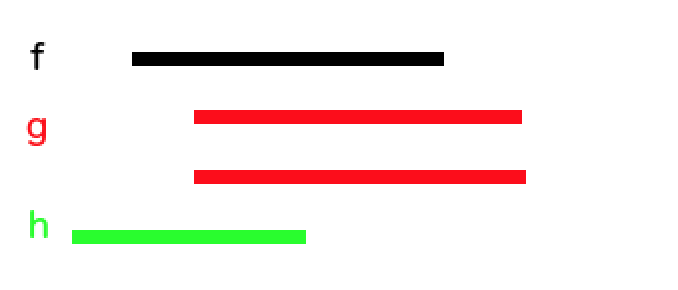
\includegraphics[scale= 0.50]{offset.png}
		\caption{Deux paires d'alignement $(f,g)$ et $(g,f)$}
		\label{fig:offset}
\end{figure}

Une telle approche, plutôt naïve, fournit déjà des résultats plutôt satisfaisants.
\end{comment}
